\chapter{Tablas, figuras, expresiones matemáticas y algoritmos}
\chaptermark{Tablas, figuras y otros} % Cuando el título es muy largo, este comando sirve para cambiar el texto que aparece en la cabecera de las páginas pares

\section{Figuras}

Las Figuras \ref{fig:Bernoulli1} y \ref{fig:violin_besa_escenario4} muestran ejemplos de cómo insertar figuras en el TFM. Algunas herramientas como R permiten exportar las gráficas en formato latex. Cuando esto sea posible es aconsejable usar estos formatos ya que las imágenes no perderán calidad al ser aumentadas o visualizadas en pantallas grandes. Se puede ver un ejemplo de cómo conseguir esto desde R en \url{http://iltabiai.github.io/tips/latex/2015/09/15/latex-tikzdevice-r.html}. El resultado lo podemos ver en la Figura \ref{fig:variacion_fitness}.

\begin{figure*}[!htb]
	\centering
	\includegraphics[width=0.5\textwidth]{recursos/Figure2}
	\caption{Violinplot fot BESA in scenario 4}
	\label{fig:violin_besa_escenario4}
\end{figure*}

\begin{figure*}[!htb]
    \centering
    \begin{subfigure}[b]{0.5\textwidth}
        \includegraphics[width=\textwidth]{recursos/Figure1a}
        \caption{Mean cumulative regret along trials}
        \label{fig:Bernoulli1_semilog}
    \end{subfigure}
    \begin{subfigure}[b]{0.5\textwidth}
        \includegraphics[width=\textwidth]{recursos/Figure1b}
        \caption{Multiple violinplot}
        \label{fig:Bernoulli1_boxplot}
    \end{subfigure}
    \caption{Comparative of the policies for scenario 1}
    \label{fig:Bernoulli1}
\end{figure*}

\begin{figure}[!ht]
	\centering
	% Created by tikzDevice version 0.12 on 2018-12-09 20:45:12
% !TEX encoding = UTF-8 Unicode
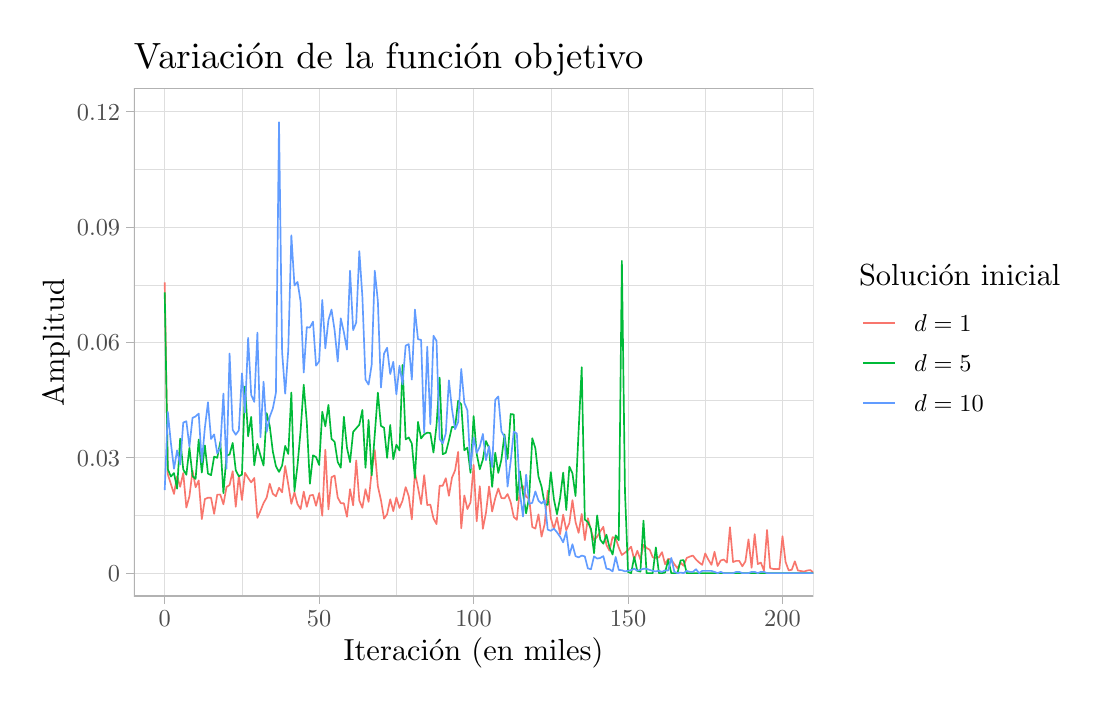
\begin{tikzpicture}[x=1pt,y=1pt]
\definecolor{fillColor}{RGB}{255,255,255}
\path[use as bounding box,fill=fillColor,fill opacity=0.00] (0,0) rectangle (384.11,236.16);
\begin{scope}
\path[clip] (  0.00,  0.00) rectangle (384.11,236.16);
\definecolor{drawColor}{RGB}{255,255,255}
\definecolor{fillColor}{RGB}{255,255,255}

\path[draw=drawColor,line width= 0.6pt,line join=round,line cap=round,fill=fillColor] (  0.00,  0.00) rectangle (384.11,236.16);
\end{scope}
\begin{scope}
\path[clip] ( 38.36, 30.72) rectangle (283.91,214.12);
\definecolor{fillColor}{RGB}{255,255,255}

\path[fill=fillColor] ( 38.36, 30.72) rectangle (283.91,214.12);
\definecolor{drawColor}{gray}{0.87}

\path[draw=drawColor,line width= 0.1pt,line join=round] ( 38.36, 59.90) --
	(283.91, 59.90);

\path[draw=drawColor,line width= 0.1pt,line join=round] ( 38.36,101.58) --
	(283.91,101.58);

\path[draw=drawColor,line width= 0.1pt,line join=round] ( 38.36,143.26) --
	(283.91,143.26);

\path[draw=drawColor,line width= 0.1pt,line join=round] ( 38.36,184.95) --
	(283.91,184.95);

\path[draw=drawColor,line width= 0.1pt,line join=round] ( 77.42, 30.72) --
	( 77.42,214.12);

\path[draw=drawColor,line width= 0.1pt,line join=round] (133.23, 30.72) --
	(133.23,214.12);

\path[draw=drawColor,line width= 0.1pt,line join=round] (189.04, 30.72) --
	(189.04,214.12);

\path[draw=drawColor,line width= 0.1pt,line join=round] (244.84, 30.72) --
	(244.84,214.12);

\path[draw=drawColor,line width= 0.3pt,line join=round] ( 38.36, 39.06) --
	(283.91, 39.06);

\path[draw=drawColor,line width= 0.3pt,line join=round] ( 38.36, 80.74) --
	(283.91, 80.74);

\path[draw=drawColor,line width= 0.3pt,line join=round] ( 38.36,122.42) --
	(283.91,122.42);

\path[draw=drawColor,line width= 0.3pt,line join=round] ( 38.36,164.11) --
	(283.91,164.11);

\path[draw=drawColor,line width= 0.3pt,line join=round] ( 38.36,205.79) --
	(283.91,205.79);

\path[draw=drawColor,line width= 0.3pt,line join=round] ( 49.52, 30.72) --
	( 49.52,214.12);

\path[draw=drawColor,line width= 0.3pt,line join=round] (105.33, 30.72) --
	(105.33,214.12);

\path[draw=drawColor,line width= 0.3pt,line join=round] (161.13, 30.72) --
	(161.13,214.12);

\path[draw=drawColor,line width= 0.3pt,line join=round] (216.94, 30.72) --
	(216.94,214.12);

\path[draw=drawColor,line width= 0.3pt,line join=round] (272.75, 30.72) --
	(272.75,214.12);
\definecolor{drawColor}{RGB}{248,118,109}

\path[draw=drawColor,line width= 0.6pt,line join=round] ( 49.52,144.12) --
	( 50.64, 74.79) --
	( 51.76, 71.22) --
	( 52.87, 67.68) --
	( 53.99, 74.05) --
	( 55.10, 70.27) --
	( 56.22, 75.24) --
	( 57.34, 62.75) --
	( 58.45, 66.82) --
	( 59.57, 76.08) --
	( 60.68, 70.08) --
	( 61.80, 72.54) --
	( 62.92, 58.57) --
	( 64.03, 65.81) --
	( 65.15, 66.32) --
	( 66.26, 66.29) --
	( 67.38, 60.48) --
	( 68.50, 67.41) --
	( 69.61, 67.45) --
	( 70.73, 63.92) --
	( 71.85, 70.20) --
	( 72.96, 70.89) --
	( 74.08, 75.87) --
	( 75.19, 63.04) --
	( 76.31, 74.45) --
	( 77.43, 65.48) --
	( 78.54, 75.29) --
	( 79.66, 73.47) --
	( 80.77, 71.84) --
	( 81.89, 73.45) --
	( 83.01, 59.01) --
	( 84.12, 61.58) --
	( 85.24, 64.37) --
	( 86.35, 66.33) --
	( 87.47, 71.37) --
	( 88.59, 67.72) --
	( 89.70, 66.82) --
	( 90.82, 69.89) --
	( 91.94, 68.28) --
	( 93.05, 77.77) --
	( 94.17, 71.12) --
	( 95.28, 64.11) --
	( 96.40, 68.27) --
	( 97.52, 63.93) --
	( 98.63, 62.21) --
	( 99.75, 68.51) --
	(100.86, 63.01) --
	(101.98, 67.11) --
	(103.10, 67.35) --
	(104.21, 63.39) --
	(105.33, 68.00) --
	(106.45, 59.82) --
	(107.56, 83.65) --
	(108.68, 62.11) --
	(109.79, 73.70) --
	(110.91, 74.31) --
	(112.03, 66.36) --
	(113.14, 64.34) --
	(114.26, 64.29) --
	(115.37, 59.42) --
	(116.49, 69.39) --
	(117.61, 63.56) --
	(118.72, 79.80) --
	(119.84, 65.29) --
	(120.95, 62.67) --
	(122.07, 69.40) --
	(123.19, 64.79) --
	(124.30, 75.75) --
	(125.42, 83.58) --
	(126.54, 70.47) --
	(127.65, 65.47) --
	(128.77, 58.74) --
	(129.88, 60.34) --
	(131.00, 65.75) --
	(132.12, 61.46) --
	(133.23, 66.43) --
	(134.35, 62.62) --
	(135.46, 65.25) --
	(136.58, 70.15) --
	(137.70, 66.86) --
	(138.81, 58.48) --
	(139.93, 75.57) --
	(141.04, 70.01) --
	(142.16, 64.00) --
	(143.28, 74.47) --
	(144.39, 63.66) --
	(145.51, 63.82) --
	(146.63, 58.81) --
	(147.74, 56.79) --
	(148.86, 70.66) --
	(149.97, 70.63) --
	(151.09, 73.35) --
	(152.21, 67.01) --
	(153.32, 73.56) --
	(154.44, 76.19) --
	(155.55, 82.91) --
	(156.67, 55.27) --
	(157.79, 67.10) --
	(158.90, 62.21) --
	(160.02, 64.65) --
	(161.14, 78.21) --
	(162.25, 57.81) --
	(163.37, 70.48) --
	(164.48, 55.08) --
	(165.60, 60.85) --
	(166.72, 70.35) --
	(167.83, 61.33) --
	(168.95, 66.09) --
	(170.06, 69.65) --
	(171.18, 66.21) --
	(172.30, 66.06) --
	(173.41, 67.64) --
	(174.53, 64.72) --
	(175.64, 59.40) --
	(176.76, 58.29) --
	(177.88, 69.72) --
	(178.99, 70.51) --
	(180.11, 66.72) --
	(181.23, 65.91) --
	(182.34, 55.72) --
	(183.46, 55.16) --
	(184.57, 60.29) --
	(185.69, 52.26) --
	(186.81, 56.78) --
	(187.92, 68.88) --
	(189.04, 58.93) --
	(190.15, 55.09) --
	(191.27, 59.11) --
	(192.39, 53.17) --
	(193.50, 60.18) --
	(194.62, 54.57) --
	(195.73, 57.12) --
	(196.85, 65.43) --
	(197.97, 57.49) --
	(199.08, 53.60) --
	(200.20, 60.44) --
	(201.32, 50.98) --
	(202.43, 58.90) --
	(203.55, 54.45) --
	(204.66, 50.98) --
	(205.78, 52.21) --
	(206.90, 54.15) --
	(208.01, 55.80) --
	(209.13, 49.22) --
	(210.24, 47.17) --
	(211.36, 52.10) --
	(212.48, 51.56) --
	(213.59, 48.30) --
	(214.71, 45.61) --
	(215.83, 46.46) --
	(216.94, 47.38) --
	(218.06, 48.62) --
	(219.17, 43.87) --
	(220.29, 47.15) --
	(221.41, 44.01) --
	(222.52, 49.32) --
	(223.64, 48.15) --
	(224.75, 47.54) --
	(225.87, 44.77) --
	(226.99, 44.54) --
	(228.10, 44.78) --
	(229.22, 46.64) --
	(230.33, 42.27) --
	(231.45, 44.22) --
	(232.57, 43.95) --
	(233.68, 42.26) --
	(234.80, 40.85) --
	(235.92, 42.82) --
	(237.03, 41.74) --
	(238.15, 44.56) --
	(239.26, 45.03) --
	(240.38, 45.41) --
	(241.50, 43.97) --
	(242.61, 42.93) --
	(243.73, 42.06) --
	(244.84, 46.18) --
	(245.96, 43.94) --
	(247.08, 42.06) --
	(248.19, 46.77) --
	(249.31, 41.63) --
	(250.42, 43.63) --
	(251.54, 43.98) --
	(252.66, 42.87) --
	(253.77, 55.65) --
	(254.89, 43.07) --
	(256.01, 43.48) --
	(257.12, 43.49) --
	(258.24, 41.53) --
	(259.35, 43.31) --
	(260.47, 51.26) --
	(261.59, 41.00) --
	(262.70, 53.14) --
	(263.82, 42.34) --
	(264.93, 42.87) --
	(266.05, 40.00) --
	(267.17, 54.65) --
	(268.28, 40.86) --
	(269.40, 40.58) --
	(270.52, 40.52) --
	(271.63, 40.55) --
	(272.75, 52.39) --
	(273.86, 43.12) --
	(274.98, 40.05) --
	(276.10, 40.27) --
	(277.21, 43.32) --
	(278.33, 40.01) --
	(279.44, 39.81) --
	(280.56, 39.62) --
	(281.68, 40.00) --
	(282.79, 40.17) --
	(283.91, 39.32) --
	(285.02, 39.77) --
	(286.14, 39.68) --
	(287.26, 39.31) --
	(288.37, 39.91) --
	(289.49, 39.44) --
	(290.61, 39.29) --
	(291.72, 45.30) --
	(292.84, 56.34) --
	(293.95, 41.16) --
	(295.07, 39.18) --
	(296.19, 61.21) --
	(297.30, 39.67) --
	(298.42, 39.06) --
	(299.53, 43.90) --
	(300.65, 39.20) --
	(301.77, 39.13) --
	(302.88, 39.29) --
	(304.00, 39.29) --
	(305.11, 39.15) --
	(306.23, 39.29) --
	(307.35, 39.13) --
	(308.46, 39.20) --
	(309.58, 39.20) --
	(310.70, 39.06) --
	(311.81, 39.06) --
	(312.93, 43.30) --
	(314.04, 39.08) --
	(315.16, 39.29) --
	(316.28, 39.06) --
	(317.39, 39.06) --
	(318.51, 39.22) --
	(319.62, 39.06) --
	(320.74, 39.41) --
	(321.86, 39.06) --
	(322.97, 39.06) --
	(324.09, 39.06) --
	(325.20, 39.06) --
	(326.32, 39.15) --
	(327.44, 39.06) --
	(328.55, 39.08) --
	(329.67, 39.13) --
	(330.79, 39.06) --
	(331.90, 39.06) --
	(333.02, 39.06) --
	(334.13, 39.06) --
	(335.25, 39.06) --
	(336.37, 39.06) --
	(337.48, 39.06) --
	(338.60, 39.13) --
	(339.71, 39.06) --
	(340.83, 39.06) --
	(341.95, 39.06) --
	(343.06, 39.13) --
	(344.18, 39.06) --
	(345.30, 39.06) --
	(346.41, 39.06) --
	(347.53, 39.06) --
	(348.64, 39.06) --
	(349.76, 39.06) --
	(350.88, 39.06) --
	(351.99, 39.06) --
	(353.11, 39.06) --
	(354.22, 39.06) --
	(355.34, 39.06) --
	(356.46, 39.06) --
	(357.57, 39.18) --
	(358.69, 39.06) --
	(359.80, 39.06) --
	(360.92, 39.06) --
	(362.04, 39.06) --
	(363.15, 39.06) --
	(364.27, 39.06) --
	(365.39, 39.20) --
	(366.50, 39.06) --
	(367.62, 39.06) --
	(368.73, 39.11) --
	(369.85, 39.06) --
	(370.97, 39.06) --
	(372.08, 39.06) --
	(373.20, 39.06) --
	(374.31, 39.06) --
	(375.43, 39.06) --
	(376.55, 39.06) --
	(377.66, 39.06) --
	(378.78, 39.06) --
	(379.89, 39.06) --
	(381.01, 39.06) --
	(382.13, 39.06) --
	(383.24, 39.06) --
	(384.11, 39.06);
\definecolor{drawColor}{RGB}{0,186,56}

\path[draw=drawColor,line width= 0.6pt,line join=round] ( 49.52,140.47) --
	( 50.64, 76.59) --
	( 51.76, 73.97) --
	( 52.87, 75.22) --
	( 53.99, 69.57) --
	( 55.10, 87.66) --
	( 56.22, 76.52) --
	( 57.34, 74.61) --
	( 58.45, 84.34) --
	( 59.57, 74.15) --
	( 60.68, 73.10) --
	( 61.80, 87.33) --
	( 62.92, 75.40) --
	( 64.03, 85.23) --
	( 65.15, 75.03) --
	( 66.26, 74.44) --
	( 67.38, 81.14) --
	( 68.50, 80.71) --
	( 69.61, 86.50) --
	( 70.73, 67.95) --
	( 71.85, 81.57) --
	( 72.96, 81.93) --
	( 74.08, 86.10) --
	( 75.19, 76.23) --
	( 76.31, 74.04) --
	( 77.43, 74.64) --
	( 78.54,106.48) --
	( 79.66, 88.49) --
	( 80.77, 95.52) --
	( 81.89, 78.05) --
	( 83.01, 85.75) --
	( 84.12, 81.57) --
	( 85.24, 77.94) --
	( 86.35, 96.85) --
	( 87.47, 92.20) --
	( 88.59, 82.99) --
	( 89.70, 77.70) --
	( 90.82, 75.64) --
	( 91.94, 77.90) --
	( 93.05, 85.03) --
	( 94.17, 82.12) --
	( 95.28,104.33) --
	( 96.40, 68.64) --
	( 97.52, 78.14) --
	( 98.63, 90.66) --
	( 99.75,107.11) --
	(100.86, 93.59) --
	(101.98, 71.35) --
	(103.10, 81.64) --
	(104.21, 80.97) --
	(105.33, 78.14) --
	(106.45, 97.39) --
	(107.56, 92.09) --
	(108.68, 99.84) --
	(109.79, 87.56) --
	(110.91, 86.53) --
	(112.03, 79.20) --
	(113.14, 77.15) --
	(114.26, 95.57) --
	(115.37, 84.42) --
	(116.49, 79.17) --
	(117.61, 90.10) --
	(118.72, 91.39) --
	(119.84, 92.68) --
	(120.95, 98.03) --
	(122.07, 77.11) --
	(123.19, 94.40) --
	(124.30, 74.42) --
	(125.42, 89.13) --
	(126.54,104.26) --
	(127.65, 92.28) --
	(128.77, 91.59) --
	(129.88, 80.70) --
	(131.00, 92.59) --
	(132.12, 80.23) --
	(133.23, 85.47) --
	(134.35, 83.38) --
	(135.46,114.28) --
	(136.58, 87.37) --
	(137.70, 88.09) --
	(138.81, 85.89) --
	(139.93, 73.43) --
	(141.04, 93.71) --
	(142.16, 87.72) --
	(143.28, 89.20) --
	(144.39, 89.81) --
	(145.51, 89.67) --
	(146.63, 82.62) --
	(147.74, 92.52) --
	(148.86,109.69) --
	(149.97, 82.03) --
	(151.09, 82.56) --
	(152.21, 87.01) --
	(153.32, 91.92) --
	(154.44, 91.74) --
	(155.55,101.34) --
	(156.67,100.04) --
	(157.79, 83.45) --
	(158.90, 84.42) --
	(160.02, 75.31) --
	(161.14, 95.82) --
	(162.25, 82.18) --
	(163.37, 76.60) --
	(164.48, 80.08) --
	(165.60, 86.80) --
	(166.72, 84.28) --
	(167.83, 70.23) --
	(168.95, 82.54) --
	(170.06, 75.28) --
	(171.18, 80.11) --
	(172.30, 89.17) --
	(173.41, 80.32) --
	(174.53, 96.54) --
	(175.64, 96.40) --
	(176.76, 65.35) --
	(177.88, 75.86) --
	(178.99, 67.78) --
	(180.11, 60.63) --
	(181.23, 66.75) --
	(182.34, 87.81) --
	(183.46, 84.14) --
	(184.57, 73.96) --
	(185.69, 70.31) --
	(186.81, 64.00) --
	(187.92, 63.75) --
	(189.04, 75.57) --
	(190.15, 65.74) --
	(191.27, 60.33) --
	(192.39, 66.15) --
	(193.50, 75.40) --
	(194.62, 61.87) --
	(195.73, 77.56) --
	(196.85, 75.14) --
	(197.97, 66.91) --
	(199.08, 90.42) --
	(200.20,113.44) --
	(201.32, 58.42) --
	(202.43, 57.51) --
	(203.55, 55.02) --
	(204.66, 46.27) --
	(205.78, 59.93) --
	(206.90, 51.15) --
	(208.01, 49.69) --
	(209.13, 52.93) --
	(210.24, 48.37) --
	(211.36, 45.79) --
	(212.48, 52.73) --
	(213.59, 50.95) --
	(214.71,151.90) --
	(215.83, 68.71) --
	(216.94, 39.46) --
	(218.06, 39.06) --
	(219.17, 44.90) --
	(220.29, 39.87) --
	(221.41, 39.61) --
	(222.52, 58.04) --
	(223.64, 39.06) --
	(224.75, 39.06) --
	(225.87, 39.06) --
	(226.99, 48.37) --
	(228.10, 39.06) --
	(229.22, 39.06) --
	(230.33, 39.26) --
	(231.45, 43.84) --
	(232.57, 39.06) --
	(233.68, 39.06) --
	(234.80, 39.06) --
	(235.92, 43.64) --
	(237.03, 43.74) --
	(238.15, 39.06) --
	(239.26, 39.06) --
	(240.38, 39.06) --
	(241.50, 39.06) --
	(242.61, 39.06) --
	(243.73, 39.06) --
	(244.84, 39.06) --
	(245.96, 39.06) --
	(247.08, 39.06) --
	(248.19, 39.06) --
	(249.31, 39.06) --
	(250.42, 39.06) --
	(251.54, 39.06) --
	(252.66, 39.06) --
	(253.77, 39.06) --
	(254.89, 39.06) --
	(256.01, 39.06) --
	(257.12, 39.06) --
	(258.24, 39.06) --
	(259.35, 39.06) --
	(260.47, 39.06) --
	(261.59, 39.06) --
	(262.70, 39.06) --
	(263.82, 39.06) --
	(264.93, 39.06) --
	(266.05, 39.06) --
	(267.17, 39.06) --
	(268.28, 39.06) --
	(269.40, 39.06) --
	(270.52, 39.06) --
	(271.63, 39.06) --
	(272.75, 39.06) --
	(273.86, 39.06) --
	(274.98, 39.06) --
	(276.10, 39.06) --
	(277.21, 39.06) --
	(278.33, 39.06) --
	(279.44, 39.06) --
	(280.56, 39.06) --
	(281.68, 39.06) --
	(282.79, 39.06) --
	(283.91, 39.06) --
	(285.02, 39.06) --
	(286.14, 39.06) --
	(287.26, 39.06) --
	(288.37, 39.06) --
	(289.49, 39.06) --
	(290.61, 39.06) --
	(291.72, 39.06) --
	(292.84, 39.06) --
	(293.95, 39.06) --
	(295.07, 39.06) --
	(296.19, 39.06) --
	(297.30, 39.06) --
	(298.42, 39.06) --
	(299.53, 39.06) --
	(300.65, 39.06) --
	(301.77, 39.06) --
	(302.88, 39.06) --
	(304.00, 39.06) --
	(305.11, 39.06) --
	(306.23, 39.06) --
	(307.35, 48.32) --
	(308.46, 39.06) --
	(309.58, 39.06) --
	(310.70, 39.06) --
	(311.81, 39.06) --
	(312.93, 39.06) --
	(314.04, 39.06) --
	(315.16, 39.06) --
	(316.28, 39.06) --
	(317.39, 39.06) --
	(318.51, 39.06) --
	(319.62, 39.06) --
	(320.74, 39.06) --
	(321.86, 39.06) --
	(322.97, 39.06) --
	(324.09, 39.06) --
	(325.20, 39.06) --
	(326.32, 39.06) --
	(327.44, 39.06) --
	(328.55, 39.06) --
	(329.67, 39.06) --
	(330.79, 39.06) --
	(331.90, 39.06) --
	(333.02, 39.06) --
	(334.13, 39.06) --
	(335.25, 39.06) --
	(336.37, 39.06) --
	(337.48, 39.06) --
	(338.60, 39.06) --
	(339.71, 39.06) --
	(340.83, 39.06) --
	(341.95, 43.69) --
	(343.06, 43.69) --
	(344.18, 39.06) --
	(345.30, 39.06) --
	(346.41, 39.06) --
	(347.53, 39.06) --
	(348.64, 39.06) --
	(349.76, 39.06) --
	(350.88, 39.06) --
	(351.99, 39.06) --
	(353.11, 39.06) --
	(354.22, 39.06) --
	(355.34, 39.06) --
	(356.46, 39.06) --
	(357.57, 39.06) --
	(358.69, 48.32) --
	(359.80, 39.06) --
	(360.92, 39.06) --
	(362.04, 39.06) --
	(363.15, 39.06) --
	(364.27, 39.06) --
	(365.39, 39.06) --
	(366.50, 39.06) --
	(367.62, 39.06) --
	(368.73, 39.06) --
	(369.85, 39.06) --
	(370.97, 39.06) --
	(372.08, 39.06) --
	(373.20, 39.06) --
	(374.31, 39.06);
\definecolor{drawColor}{RGB}{97,156,255}

\path[draw=drawColor,line width= 0.6pt,line join=round] ( 49.52, 69.09) --
	( 50.64, 97.31) --
	( 51.76, 86.01) --
	( 52.87, 76.76) --
	( 53.99, 83.43) --
	( 55.10, 78.27) --
	( 56.22, 93.47) --
	( 57.34, 93.94) --
	( 58.45, 84.79) --
	( 59.57, 95.17) --
	( 60.68, 95.68) --
	( 61.80, 96.73) --
	( 62.92, 79.14) --
	( 64.03, 91.58) --
	( 65.15,100.79) --
	( 66.26, 87.53) --
	( 67.38, 89.19) --
	( 68.50, 82.34) --
	( 69.61, 84.61) --
	( 70.73,103.95) --
	( 71.85, 76.79) --
	( 72.96,118.42) --
	( 74.08, 90.83) --
	( 75.19, 89.08) --
	( 76.31, 90.65) --
	( 77.43,111.24) --
	( 78.54, 97.08) --
	( 79.66,124.05) --
	( 80.77,103.43) --
	( 81.89,100.96) --
	( 83.01,125.96) --
	( 84.12, 88.18) --
	( 85.24,108.21) --
	( 86.35, 90.08) --
	( 87.47, 95.58) --
	( 88.59, 98.56) --
	( 89.70,104.21) --
	( 90.82,201.98) --
	( 91.94,118.95) --
	( 93.05,103.90) --
	( 94.17,119.81) --
	( 95.28,161.14) --
	( 96.40,143.01) --
	( 97.52,144.27) --
	( 98.63,137.12) --
	( 99.75,111.55) --
	(100.86,127.91) --
	(101.98,127.81) --
	(103.10,129.92) --
	(104.21,114.02) --
	(105.33,115.58) --
	(106.45,137.78) --
	(107.56,120.26) --
	(108.68,130.48) --
	(109.79,134.30) --
	(110.91,126.80) --
	(112.03,115.53) --
	(113.14,131.13) --
	(114.26,126.10) --
	(115.37,119.81) --
	(116.49,148.35) --
	(117.61,126.85) --
	(118.72,129.62) --
	(119.84,155.40) --
	(120.95,138.88) --
	(122.07,108.98) --
	(123.19,107.17) --
	(124.30,114.32) --
	(125.42,148.35) --
	(126.54,137.32) --
	(127.65,106.11) --
	(128.77,118.40) --
	(129.88,120.51) --
	(131.00,111.00) --
	(132.12,115.43) --
	(133.23,103.65) --
	(134.35,114.02) --
	(135.46,107.27) --
	(136.58,121.27) --
	(137.70,121.82) --
	(138.81,108.98) --
	(139.93,134.30) --
	(141.04,123.58) --
	(142.16,123.33) --
	(143.28, 89.75) --
	(144.39,120.86) --
	(145.51, 92.87) --
	(146.63,124.84) --
	(147.74,122.98) --
	(148.86, 87.49) --
	(149.97, 85.93) --
	(151.09, 89.55) --
	(152.21,108.73) --
	(153.32, 98.31) --
	(154.44, 91.06) --
	(155.55, 93.63) --
	(156.67,112.81) --
	(157.79,100.63) --
	(158.90, 97.86) --
	(160.02, 76.97) --
	(161.14, 87.99) --
	(162.25, 82.55) --
	(163.37, 84.77) --
	(164.48, 89.35) --
	(165.60, 79.89) --
	(166.72, 84.92) --
	(167.83, 77.37) --
	(168.95,101.68) --
	(170.06,102.89) --
	(171.18, 90.31) --
	(172.30, 88.29) --
	(173.41, 70.32) --
	(174.53, 79.43) --
	(175.64, 90.21) --
	(176.76, 89.50) --
	(177.88, 67.91) --
	(178.99, 59.50) --
	(180.11, 74.65) --
	(181.23, 64.08) --
	(182.34, 64.48) --
	(183.46, 68.61) --
	(184.57, 65.24) --
	(185.69, 64.23) --
	(186.81, 65.49) --
	(187.92, 54.77) --
	(189.04, 54.36) --
	(190.15, 55.12) --
	(191.27, 53.81) --
	(192.39, 52.20) --
	(193.50, 50.19) --
	(194.62, 54.06) --
	(195.73, 45.45) --
	(196.85, 49.48) --
	(197.97, 45.20) --
	(199.08, 44.75) --
	(200.20, 45.40) --
	(201.32, 45.10) --
	(202.43, 40.77) --
	(203.55, 40.47) --
	(204.66, 45.15) --
	(205.78, 44.30) --
	(206.90, 44.55) --
	(208.01, 45.20) --
	(209.13, 40.67) --
	(210.24, 40.47) --
	(211.36, 39.67) --
	(212.48, 44.90) --
	(213.59, 40.22) --
	(214.71, 40.12) --
	(215.83, 39.67) --
	(216.94, 39.92) --
	(218.06, 40.17) --
	(219.17, 40.67) --
	(220.29, 39.92) --
	(221.41, 40.27) --
	(222.52, 40.62) --
	(223.64, 40.62) --
	(224.75, 40.22) --
	(225.87, 39.87) --
	(226.99, 39.67) --
	(228.10, 39.92) --
	(229.22, 39.51) --
	(230.33, 40.07) --
	(231.45, 40.02) --
	(232.57, 44.55) --
	(233.68, 39.51) --
	(234.80, 39.06) --
	(235.92, 39.26) --
	(237.03, 39.06) --
	(238.15, 39.87) --
	(239.26, 39.51) --
	(240.38, 39.51) --
	(241.50, 40.47) --
	(242.61, 39.06) --
	(243.73, 39.87) --
	(244.84, 39.87) --
	(245.96, 39.87) --
	(247.08, 39.87) --
	(248.19, 39.51) --
	(249.31, 39.06) --
	(250.42, 39.51) --
	(251.54, 39.06) --
	(252.66, 39.06) --
	(253.77, 39.06) --
	(254.89, 39.06) --
	(256.01, 39.51) --
	(257.12, 39.51) --
	(258.24, 39.06) --
	(259.35, 39.06) --
	(260.47, 39.06) --
	(261.59, 39.51) --
	(262.70, 39.51) --
	(263.82, 39.06) --
	(264.93, 39.51) --
	(266.05, 39.51) --
	(267.17, 39.06) --
	(268.28, 39.06) --
	(269.40, 39.06) --
	(270.52, 39.06) --
	(271.63, 39.06) --
	(272.75, 39.06) --
	(273.86, 39.06) --
	(274.98, 39.06) --
	(276.10, 39.06) --
	(277.21, 39.06) --
	(278.33, 39.06) --
	(279.44, 39.06) --
	(280.56, 39.06) --
	(281.68, 39.06) --
	(282.79, 39.06) --
	(283.91, 39.06) --
	(285.02, 39.06) --
	(286.14, 39.06) --
	(287.26, 39.06) --
	(288.37, 39.06) --
	(289.49, 39.06) --
	(290.61, 39.06) --
	(291.72, 39.06) --
	(292.84, 39.06) --
	(293.95, 39.06) --
	(295.07, 39.06) --
	(296.19, 39.06) --
	(297.30, 39.06) --
	(298.42, 39.06) --
	(299.53, 39.06) --
	(300.65, 39.06) --
	(301.77, 39.06) --
	(302.88, 39.06) --
	(304.00, 39.06) --
	(305.11, 39.06) --
	(306.23, 39.06) --
	(307.35, 39.06) --
	(308.46, 39.06) --
	(309.58, 39.06) --
	(310.70, 39.06) --
	(311.81, 39.06) --
	(312.93, 39.06) --
	(314.04, 39.06) --
	(315.16, 39.06) --
	(316.28, 39.06) --
	(317.39, 39.06) --
	(318.51, 39.06) --
	(319.62, 39.06) --
	(320.74, 39.06) --
	(321.86, 39.06) --
	(322.97, 39.06) --
	(324.09, 39.06) --
	(325.20, 39.06) --
	(326.32, 39.06) --
	(327.44, 39.06);
\definecolor{drawColor}{gray}{0.70}

\path[draw=drawColor,line width= 0.6pt,line join=round,line cap=round] ( 38.36, 30.72) rectangle (283.91,214.12);
\end{scope}
\begin{scope}
\path[clip] (  0.00,  0.00) rectangle (384.11,236.16);
\definecolor{drawColor}{gray}{0.30}

\node[text=drawColor,anchor=base east,inner sep=0pt, outer sep=0pt, scale=  0.88] at ( 33.41, 36.03) {0};

\node[text=drawColor,anchor=base east,inner sep=0pt, outer sep=0pt, scale=  0.88] at ( 33.41, 77.71) {0.03};

\node[text=drawColor,anchor=base east,inner sep=0pt, outer sep=0pt, scale=  0.88] at ( 33.41,119.39) {0.06};

\node[text=drawColor,anchor=base east,inner sep=0pt, outer sep=0pt, scale=  0.88] at ( 33.41,161.07) {0.09};

\node[text=drawColor,anchor=base east,inner sep=0pt, outer sep=0pt, scale=  0.88] at ( 33.41,202.76) {0.12};
\end{scope}
\begin{scope}
\path[clip] (  0.00,  0.00) rectangle (384.11,236.16);
\definecolor{drawColor}{gray}{0.70}

\path[draw=drawColor,line width= 0.3pt,line join=round] ( 35.61, 39.06) --
	( 38.36, 39.06);

\path[draw=drawColor,line width= 0.3pt,line join=round] ( 35.61, 80.74) --
	( 38.36, 80.74);

\path[draw=drawColor,line width= 0.3pt,line join=round] ( 35.61,122.42) --
	( 38.36,122.42);

\path[draw=drawColor,line width= 0.3pt,line join=round] ( 35.61,164.11) --
	( 38.36,164.11);

\path[draw=drawColor,line width= 0.3pt,line join=round] ( 35.61,205.79) --
	( 38.36,205.79);
\end{scope}
\begin{scope}
\path[clip] (  0.00,  0.00) rectangle (384.11,236.16);
\definecolor{drawColor}{gray}{0.70}

\path[draw=drawColor,line width= 0.3pt,line join=round] ( 49.52, 27.97) --
	( 49.52, 30.72);

\path[draw=drawColor,line width= 0.3pt,line join=round] (105.33, 27.97) --
	(105.33, 30.72);

\path[draw=drawColor,line width= 0.3pt,line join=round] (161.13, 27.97) --
	(161.13, 30.72);

\path[draw=drawColor,line width= 0.3pt,line join=round] (216.94, 27.97) --
	(216.94, 30.72);

\path[draw=drawColor,line width= 0.3pt,line join=round] (272.75, 27.97) --
	(272.75, 30.72);
\end{scope}
\begin{scope}
\path[clip] (  0.00,  0.00) rectangle (384.11,236.16);
\definecolor{drawColor}{gray}{0.30}

\node[text=drawColor,anchor=base,inner sep=0pt, outer sep=0pt, scale=  0.88] at ( 49.52, 19.71) {0};

\node[text=drawColor,anchor=base,inner sep=0pt, outer sep=0pt, scale=  0.88] at (105.33, 19.71) {50};

\node[text=drawColor,anchor=base,inner sep=0pt, outer sep=0pt, scale=  0.88] at (161.13, 19.71) {100};

\node[text=drawColor,anchor=base,inner sep=0pt, outer sep=0pt, scale=  0.88] at (216.94, 19.71) {150};

\node[text=drawColor,anchor=base,inner sep=0pt, outer sep=0pt, scale=  0.88] at (272.75, 19.71) {200};
\end{scope}
\begin{scope}
\path[clip] (  0.00,  0.00) rectangle (384.11,236.16);
\definecolor{drawColor}{RGB}{0,0,0}

\node[text=drawColor,anchor=base,inner sep=0pt, outer sep=0pt, scale=  1.10] at (161.13,  7.44) {Iteración (en miles)};
\end{scope}
\begin{scope}
\path[clip] (  0.00,  0.00) rectangle (384.11,236.16);
\definecolor{drawColor}{RGB}{0,0,0}

\node[text=drawColor,rotate= 90.00,anchor=base,inner sep=0pt, outer sep=0pt, scale=  1.10] at ( 13.08,122.42) {Amplitud};
\end{scope}
\begin{scope}
\path[clip] (  0.00,  0.00) rectangle (384.11,236.16);
\definecolor{fillColor}{RGB}{255,255,255}

\path[fill=fillColor] (294.91, 87.73) rectangle (378.61,157.11);
\end{scope}
\begin{scope}
\path[clip] (  0.00,  0.00) rectangle (384.11,236.16);
\definecolor{drawColor}{RGB}{0,0,0}

\node[text=drawColor,anchor=base west,inner sep=0pt, outer sep=0pt, scale=  1.10] at (300.41,143.07) {Solución inicial};
\end{scope}
\begin{scope}
\path[clip] (  0.00,  0.00) rectangle (384.11,236.16);
\definecolor{fillColor}{RGB}{255,255,255}

\path[fill=fillColor] (300.41,122.14) rectangle (314.86,136.59);
\end{scope}
\begin{scope}
\path[clip] (  0.00,  0.00) rectangle (384.11,236.16);
\definecolor{drawColor}{RGB}{248,118,109}

\path[draw=drawColor,line width= 0.6pt,line join=round] (301.85,129.37) -- (313.42,129.37);
\end{scope}
\begin{scope}
\path[clip] (  0.00,  0.00) rectangle (384.11,236.16);
\definecolor{fillColor}{RGB}{255,255,255}

\path[fill=fillColor] (300.41,107.69) rectangle (314.86,122.14);
\end{scope}
\begin{scope}
\path[clip] (  0.00,  0.00) rectangle (384.11,236.16);
\definecolor{drawColor}{RGB}{0,186,56}

\path[draw=drawColor,line width= 0.6pt,line join=round] (301.85,114.91) -- (313.42,114.91);
\end{scope}
\begin{scope}
\path[clip] (  0.00,  0.00) rectangle (384.11,236.16);
\definecolor{fillColor}{RGB}{255,255,255}

\path[fill=fillColor] (300.41, 93.23) rectangle (314.86,107.69);
\end{scope}
\begin{scope}
\path[clip] (  0.00,  0.00) rectangle (384.11,236.16);
\definecolor{drawColor}{RGB}{97,156,255}

\path[draw=drawColor,line width= 0.6pt,line join=round] (301.85,100.46) -- (313.42,100.46);
\end{scope}
\begin{scope}
\path[clip] (  0.00,  0.00) rectangle (384.11,236.16);
\definecolor{drawColor}{RGB}{0,0,0}

\node[text=drawColor,anchor=base west,inner sep=0pt, outer sep=0pt, scale=  0.88] at (320.36,126.34) {$d=1$};
\end{scope}
\begin{scope}
\path[clip] (  0.00,  0.00) rectangle (384.11,236.16);
\definecolor{drawColor}{RGB}{0,0,0}

\node[text=drawColor,anchor=base west,inner sep=0pt, outer sep=0pt, scale=  0.88] at (320.36,111.88) {$d=5$};
\end{scope}
\begin{scope}
\path[clip] (  0.00,  0.00) rectangle (384.11,236.16);
\definecolor{drawColor}{RGB}{0,0,0}

\node[text=drawColor,anchor=base west,inner sep=0pt, outer sep=0pt, scale=  0.88] at (320.36, 97.43) {$d=10$};
\end{scope}
\begin{scope}
\path[clip] (  0.00,  0.00) rectangle (384.11,236.16);
\definecolor{drawColor}{RGB}{0,0,0}

\node[text=drawColor,anchor=base west,inner sep=0pt, outer sep=0pt, scale=  1.32] at ( 38.36,221.57) {Variación de la función objetivo};
\end{scope}
\end{tikzpicture}

	\caption{Variación de la función objetivo en intervalos de 1000 iteraciones en el caso 8 para diferentes soluciones iniciales}
	\label{fig:variacion_fitness}
\end{figure}

\section{Expresiones matemáticas}
A continuación, se muestran algunos ejemplos de expresiones matemáticas:
\begin{equation}
\mu^*\times 25000-\frac{1}{1000}\sum_{r=1}^{1000}\sum_{i=1}^{K}\sum_{j=1}^{25000}\mu_i\times X_{i,j}^r.
\end{equation}

\begin{equation}
\mu_{\widetilde{A}}(x)=\left\{ \begin{array}{cc}
\frac{x-a_{1}}{a_{2}-a_{1}} & if\; a_{1}\leq x\leq a_{2}\\
1 & if\; a_{2}\leq x\leq a_{3}\\
\frac{x-a_{4}}{a_{3}-a_{4}} & if\; a_{3}\leq x\leq a_{4}\\
0 & otherwise
\end{array}\right. .
\end{equation}

\begin{align}
\begin{split}
\widetilde{DD}(A_{1},A_{4}) & =\widetilde{DD}(A_{1},A_{4}|P_{1})\oplus \widetilde{DD}(A_{1},A_{4}|P_{2}) \\ 
& =[\widetilde{dd}(A_{1},A_{2})\otimes \widetilde{dd}(A_{2},A_{4})]\oplus \lbrack \widetilde{dd}(A_{1},A_{3})\otimes \widetilde{dd}(A_{3},A_{4})].
\end{split}
\end{align}

\begin{itemize}
\item Si $\max \{(a_{4}-a_{1}),(b_{4}-b_{1})\}\neq 0$, entonces
\begin{align*}
S(\widetilde{A},\widetilde{B})=& 1 - ( 1 - \alpha - \beta) \times \left( 1 - \frac{\int_{0}^{1} \mu_{\widetilde{A}\cap \widetilde{B}}(x)dx} {\int_{0}^{1} \mu_{\widetilde{A}\cup \widetilde{B}}(x)dx}\right) \\
& -\alpha\frac{\sum \mid a_{i} - b_{i} \mid }{4}- \beta \frac{d[(X_{\widetilde{A} },Y_{\widetilde{A}}),(X_{\widetilde{B}} ,Y_{\widetilde{B}})]}{M},
\end{align*}

\item En caso contrario,%
\begin{align*}
S(\widetilde{A} ,\widetilde{B})=& 1- \left( \frac{1-\alpha-\beta}{2} + \alpha \right) \times
\frac{\sum \mid a_i - b_i \mid}{4} - \\
& - \left( \frac{1 - \alpha - \beta}{2} + \beta \right) \times \frac{d[(X_{\widetilde{A}},Y_{\widetilde{A}}), (X_{\widetilde{B}},Y_{\widetilde{B}})]}{M},
\end{align*}
\end{itemize}
donde $\alpha +\beta <1$, $\mu _{\widetilde{\chi }}$ es la función de pertenencia de $\widetilde{\chi}$, 
\begin{equation}
M=\underset{[0,1]\times[0,\frac{1}{2}]}{\max}\{d((x,y),(x^{\prime },y^{\prime }))\}\text{,} 
\end{equation}%
\begin{equation*}
\mu _{\widetilde{A}\cap \widetilde{B}}(x)=\underset{0\leq x\leq 1}{\min}%
\{\mu _{\widetilde{A}}(x),\mu _{\widetilde{B}}(x)\} ,
\;\;\; \mu _{\widetilde{A}\cup \widetilde{B}}(x)=\underset{0\leq x\leq 1}{\max}%
\{\mu _{\widetilde{A}}(x),\mu _{\widetilde{B}}(x)\}.
\end{equation*}%

\section{Algoritmos}

El Algoritmo \ref{getDelay} ilustra la forma que debe adoptarse. Se usa el paquete \textit{algorithmic}. Los comandos pueden consultarse en \url{https://en.wikibooks.org/wiki/LaTeX/Algorithms} o en la documentación oficial.

\begin{algorithm}[h]
	\begin{algorithmic}
	\REQUIRE $t_0$ = instante en el que se genera el retardo
	
	\IF{$(update\_architecture==1)$}
		\IF{$(delay\_scenario==1)$}
			\STATE{delay$=C$}
		\ELSE
			\IF{$(reward\_scenario==1)$}
				\STATE{delay $\leftarrow [0,300]$-trunc\_Exp($\lambda=1/80$)}
			\ELSE
				\STATE{delay $\leftarrow [0,480]$-trunc\_Exp($\lambda=1/150$)}
			\ENDIF
		\ENDIF
	\ELSE
		\STATE{delay = difference(24:00, $t_0$)}
	\ENDIF
	
	\RETURN delay
	\end{algorithmic}
	\caption{$getDelay(t_0)$}
	\label{getDelay}
\end{algorithm}

\section{Tablas}
La tabla \ref{table:results45} muestra un ejemplo de cómo poner notas a pie de tabla (necesario el paquete threeparttable). En la tabla \ref{table:risk} se usa el entorno \textit{stripedtable} para marcar la líneas alternas con diferentes colores.

\begin{table}[htb]
\begin{threeparttable}
	\centering
	\caption{Mean cumulative regrets and standard deviations}
	\label{table:results45}
	\begin{small}
	\begin{tabular}{llllll}
		\toprule
			& \multicolumn{2}{c}{Truncated Poisson} & & \multicolumn{2}{c}{Truncated Exponential} \\ 
		\cmidrule{2-3}\cmidrule{5-6}
		 	& Mean & $\sigma$ & & Mean & $\sigma$\\ \midrule
		 UCB\tnote{1} & 2632.65 & 246.03 & & 1295.79 & 514.03 \\
		 DMED+ & 978.56 & 225.24 & & \textbf{645.70} & 493.8 \\
		 KL-UCB & 1817.4 & 236.57 & & 1219.98 & 510.69 \\
		 KL-UCB poisson & \textbf{314.99*} & 201.79 & & - & - \\
		 KL-UCB exp & - & - & & 786.30 & 498.16 \\
		 KL-UCB+ & 1190.64 & 225.82 & & 813.45 & 494.59 \\
		 BESA & 2015.73 & 3561.5 & & 755.87 & 2323.22 \\
		 PR-1 & 1314.9 & 234.25 & & 660.64 & 492.37 \\ 
		 PR-2 (TS) & \textbf{917.67} & 222.79 & & \textbf{630.38} & 487.01 \\
		 PR-3 & \textbf{736.6} & 210.96 & & \textbf{565.79*} & 480.99 \\
		 \bottomrule
	\end{tabular}
	\end{small}
	\begin{tablenotes}
		\item[1] Esto es una nota a pie de tabla
	\end{tablenotes}
\end{threeparttable}
\end{table}

\begin{stripedtable}[htb]
	\centering
	\caption{Risks to $A_5$ after the implementation of the selected safeguards}
	\label{table:risk}
	\begin{scriptsize}
	\begin{tabular}{cccc}
		\toprule
		\hiderowcolors
		Threat & Confidentiality & Integrity & Authenticity \\
		\midrule
		\showrowcolors
		$T_{1}^{1}$ & (16.9, 161.72, 936.2, 3681.5) & (32.70, 239.7, 1295.6, 5197.4) & (25.1, 198.6, 1576.7, 5777.1)\\
		$T_{1}^{2}$ & (0, 49.6, 458.1, 1791.2) & (0, 29.7, 289.7, 1397.1) & (0, 24.6, 352.6, 1552.9)\\
		$T_{2}^{2}$ & (0, 49.6, 458.1, 1791.2) & (0, 29.7, 289.7, 1397.1) & (76, 379.3, 2074.3, 5588.4)\\
		$T_{1}^{3}$ & (12.2, 110.5, 647.2, 2465.6) & (21.9, 147.3, 744.3, 2958.7) & (6.8, 58.5, 487.1, 1923.2)\\ 
		$T_{1}^{4}$ & (34.8, 245.5, 1176.8, 3793.2) & (62.7, 327.4, 1353.3, 4551.9) & (19.5, 129.9, 885.7, 2958.7)\\
		\bottomrule
		\hiderowcolors
	\end{tabular}
	\end{scriptsize}
\end{stripedtable}